\begin{markdown}
#30天 LaTeX 挑戰 Day 21 Ti*k*Z

-------

##進階使用

###節點

在 TikZ 中可以利用 `\node(name) at(x,y) {text};` 放置節點

```latex
\begin{tikzpicture}
\draw[help lines] (-2,-2) grid (2,2);
\node(1) at(0,0) {原點};
\end{tikzpicture}
```

想要連接兩個節點時,可以將座標改為兩個節點的名字

```latex
\begin{tikzpicture}
\node(A) at(0,0) {A};
\node(B) at(2,0) {B};
\node(C) at(0,2) {C};
\draw (A)--(B)--(C);
\end{tikzpicture}
```

`\node `如同 `\draw `也可以使用選項來調整樣式

```latex
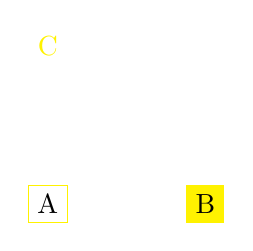
\begin{tikzpicture}
\node[draw=yellow](A) at(0,0) {A};
\node[fill=yellow](B) at(2,0) {B};
\node[text=yellow](C) at(0,2) {C};
\end{tikzpicture}
```

當然也有一些是只能用在 `\node `上的選項

```latex
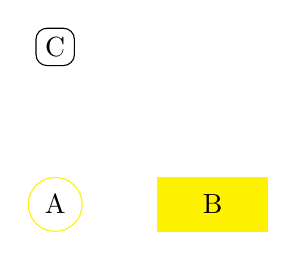
\begin{tikzpicture}
\node[draw=yellow,circle](A) at(0,0) {A};
\node[fill=yellow, minimum width=40pt, minimum height=20pt](B) at(2,0) {B};
\node[draw=black, rounded corners](C) at(0,2) {C};
\end{tikzpicture}
```

* 第一個節點用 circle 將外匡變成圓形的
* 第二個節點用 minimum width/height 定義節點的最小長寬
* 第三個節點用 rounded corners 把節點的邊角轉成圓角

但有時候我們並不想要直接把節點放到指定的座標,而是想放到該座標的上下左右,這個時候也可以利用 TikZ 內建的選項來達成

```latex

\begin{tikzpicture}
\node[left] at(0,0) {left};
\node[right] at(0,0) {right};
\node[above] at(0,0) {above};
\node[below] at(0,0) {below};
\draw[fill=black] (0,0) circle (.1);
\end{tikzpicture}
```

* 第一個節點在 (0,0) 的左邊
* 第二個節點在 (0,0) 的右邊
* 第三個節點在 (0,0) 的上方
* 第四個節點在 (0,0) 的下方

###自定義樣式

如果你圖片裡的節點畫線條都有相似的共同點,你可以在`\begin {tikzpicture}` 後加一個方括號,並將共通的選項放在方括號中

```latex
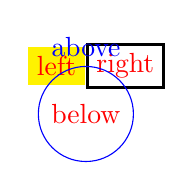
\begin{tikzpicture}[text = red]
\node[left, fill = yellow] at(0,0) {left};
\node[right, draw = black, line width =1pt] at(0,0) {right};
\node[above, text = blue] at(0,0) {above};
\node[below, draw = blue, circle] at(0,0) {below};
\end{tikzpicture}
```

如果你有一個很複雜的樣式,但又不是共通的,你可以利用`\tikzset{}`來將複雜的樣式定義成一個選項

```latex
\tikzset{mynode/.style = {
draw = gray!70!black,
line width = 0.8pt,
fill = blue!30,
rounded corners,
inner sep = 6pt, %文字與邊匡的距離
minimum width = 40pt,
minimum height = 20pt}
}
```

使用時只要用 `\node[mynode]` 即可

```latex

\begin{tikzpicture}[->, line width = 2pt]
\node[mynode] (1) at (0,0) {First Thing};
\node[mynode] (2) at (3,0) {Second Thing};
\node[mynode] (3) at (6,0) {Third Thing};
\draw (1)--(2);
\draw (2)--(3);
\end{tikzpicture}
```

這樣就方便許多了

###函數圖

畫函數一樣是使用`\draw ` 這個命令

```latex
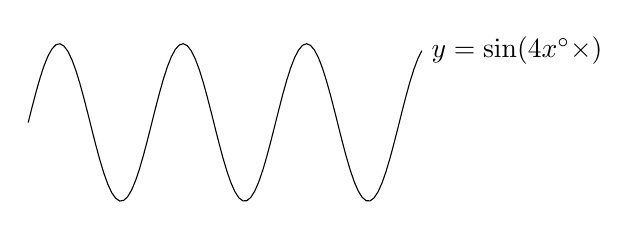
\begin{tikzpicture}
\draw[domain = 0:5, samples = 100] plot (\x,{sin(deg(\x*4))}) node[right] {$y=\sin(4x^\circ \times)$};
\end{tikzpicture}
```

domain 是我們要畫的區間,起點與終點要用冒號隔開,samples 決定圖形的精細程度,要特別注意的是需要運算的部分需要放在`{}`之間

![TikZ](TikZ)

上圖是可以使用的運算子,不過更複雜的函數圖形 TikZ 就很難畫出來了,所以下一篇會介紹 pgfplot 這個 package

\end{markdown}
